\documentclass[11pt,twoside,a4paper]{article}

\usepackage[italian]{babel}
\usepackage{listings}
\usepackage{color}
\usepackage{mathtools}
\usepackage{biblatex}
%useful colors
\definecolor{mygreen}{rgb}{0,0.6,0}
\definecolor{mygray}{rgb}{0.5,0.5,0.5}
\definecolor{mymauve}{rgb}{0.58,0,0.82}
\definecolor{gray}{rgb}{0.4,0.4,0.4}
\definecolor{darkblue}{rgb}{0.0,0.0,0.6}
\definecolor{cyan}{rgb}{0.0,0.6,0.6}
%defining styles for listings
%java listings
\lstdefinestyle{java}{
	basicstyle=\footnotesize,
	breakatwhitespace=false,
	breaklines=true,
	captionpos=b,
	commentstyle=\color{mygreen},
	frame=single,
	keywordstyle=\color{blue},
	language=java,
	numbers=left,
	numbersep=5pt,
	numberstyle=\tiny\color{mygray},
	rulecolor=\color{black},
	showstringspaces=false,
	stepnumber=1,
	stringstyle=\color{mymauve},
	tabsize=2,
	title=\lstname
}
%javascript listings
\lstdefinestyle{javascript}{
	basicstyle=\footnotesize,
	breakatwhitespace=false,
	breaklines=true,
	captionpos=b,
	commentstyle=\color{mygreen},
	frame=single,
	keywordstyle=\color{blue},
	language=javascript,
	numbers=left,
	numbersep=5pt,
	numberstyle=\tiny\color{mygray},
	rulecolor=\color{black},
	showstringspaces=false,
	stepnumber=1,
	stringstyle=\color{mymauve},
	tabsize=2,
	title=\lstname
}
%php listings
\lstdefinestyle{php}{
	basicstyle=\footnotesize,
	breakatwhitespace=false,
	breaklines=true,
	captionpos=b,
	commentstyle=\color{mygreen},
	frame=single,
	keywordstyle=\color{blue},
	language=php,
	numbers=left,
	numbersep=5pt,
	numberstyle=\tiny\color{mygray},
	rulecolor=\color{black},
	showstringspaces=false,
	stepnumber=1,
	stringstyle=\color{mymauve},
	tabsize=2,
	title=\lstname
}
%xml listings
\lstdefinelanguage{XML}
{
	morestring=[b]",
	morestring=[s]{>}{<},
	morecomment=[s]{<?}{?>},
	stringstyle=\color{black},
	identifierstyle=\color{darkblue},
	keywordstyle=\color{cyan},
	morekeywords={xmlns,version,type}% list your attributes here
}


\lstdefinestyle{xml}{
	basicstyle=\ttfamily,
	breakatwhitespace=false,
	breaklines=true,
	columns=fullflexible,
	showstringspaces=false,
	captionpos=b,
	commentstyle=\color{mygreen},
	frame=single,
	keywordstyle=\color{blue},
	language=XML,
	numbers=none,
	rulecolor=\color{black},
	tabsize=4,
	title=\lstname
}
\begin{document}
\title{Finding similar papers using ontologies}
\author{Francesco Gaetano, Luigi Lomasto, Marco Mecchia, Andrea Sold\'a }
\date{Gennaio 2016}
\maketitle
\section{Introduzione al problema}
Il problema di trovare lavori scientifici simili scritti in linguaggio naturale \'e un compito molto difficile dal punto di vista informatico: Tali documenti infatti non hanno una struttura fissa, e sono pieni  di elementi non facilmente confrontabili come formule, notazioni ed immagini. Inoltre, nonostante una netta predominanza dell'inglese, i documenti sono scritti in lingue diverse. Tutte queste caratteristiche, insite in lavori di ricerca di questo tipo, rendono gli approcci basati sul confronto testuale non utilizzabili. Il nostro lavoro, basato sulle meta informazioni dei documenti e sull'utilizzo di tecnologie del Semantic Web, mira a fornire un approccio alternativo ai metodi tradizionali, nonch\'e un'infrastruttura riutilizzabile anche in altri ambiti.

Il resto del lavoro \'e organizzato come segue: nella sezione \ref{sec:workflow} viene presentata l'analisi da noi condotta ed i vari step che hanno portato al risultato finale. Nella sezione \ref{sec:tools} vengono analizzati nel dettaglio le tecnologie del Web Semantico da noi utilizzate. Nella sezione \ref{sec:implementation} vengono presentate nel dettaglio le varie componenti introdotte nella sezione \ref{sec:workflow}, illustrando e commentando estratti di codice del progetto. Infine, nella sezione \ref{sec:conclusions} verranno commentati i risultati ottenuti ed eventuali applicazioni ed estensioni di quanto fatto.

\section{Workflow}
\label{sec:workflow}
Il lavoro \'e stato suddiviso in diverse fasi. 

\subsection{Selezione del database ed estrazione delle meta-informazioni}
\label{subsec:infoextraction}
In questa fase preliminare del lavoro, abbiamo costruito il dataset sul quale basarci per tutto il resto del lavoro. Per prima cosa abbiamo scelto il database dal quale attingere i lavori da confrontare. La nostra scelta e' ricaduta su DBLP\cite{DBLP} in quanto punto di riferimento centrale per la sottomissione dei paper nella comunita' informatica. DBLP inoltre mette a disposizione ampi dataset di meta-informazioni sugli articoli scaricabili in formato standard xml, con relativi url alle pagine web degli articoli.
Tramite gli url, abbiamo estratto dalle pagine web gli abstract di ogni articolo tramite \emph{scraping}. Nel nostro dataset finale, ogni articolo ha quindi i seguenti campi:
\begin{itemize}
	\item Titolo del lavoro
	\item Autori del lavoro
	\item Anno di pubblicazione
	\item Abstract
	\item Topics (se presenti)
	\item Keyword (se presenti)
	\item Rivista
	\item URL
\end{itemize} 
Inoltre, attraverso l'utilizzo del estrattore di keywords AlchemyAPI, dagli abstract sono state estratte le parole chiave con relativa rilevanza all'interno dell'articolo. Queste keyword sono state aggiunte a quelle gi\'a esistenti.

\subsection{Progettazione e popolamento dell'ontologia}
\label{subsec:ontology}
In questa fase, \'e stata studiata la progettazione di un'ontologia adatta a gestire le informazioni estratte nella fase precedente. Il passaggio ad un'ontologia \'e stato necessario per almeno due motivi:
\begin{enumerate}
	\item La possibilit\'a di interrogare il database di meta informazioni tramite query semantiche.
	\item La possibilit\'a di collegare il lavoro a strumenti gi\'a esistenti per i \emph{linked data}, in modo da rendere lo strumento integrabile.
\end{enumerate}
Per l'ontologia, la nostra scelta \'e ricaduta su CIDOC/CRM\cite{CIDOC}. Il modello concettuale CIDOC/CRM \'e un stato progettato per la gestione di contenuti relativi alla storia ed alle opere d'arte, quindi si \'e rivelato adatto al nostro scopo. 
Per definizione, un'onotologia \'e CRM compatibile se rispetta lo schema di base (illustrato in seguito) proposto dagli autori.
Per rappresentare in modo corretto le informazioni estratte da DBLP \'e stato necessario aggiungere, allo schema di base del CRM, altre classi e propriet\'a.  \newline

\begin{figure}
\centering
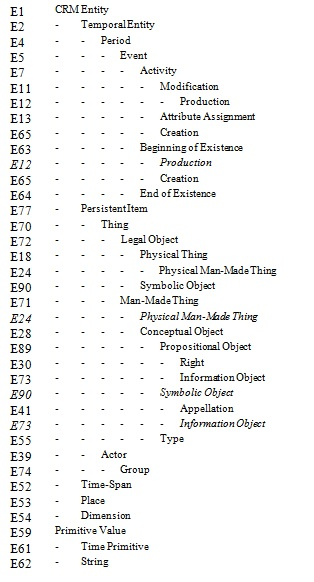
\includegraphics[scale=1.50]{immaginiTesina/ridotto.jpg}
\end{figure}



-----------Qui c\'e da appronfondire sullo schema che abbiamo progettato noi a partire dalle meta informazioni Francesco-----

\subsection{Interrogazione dell'ontologia}
\label{subsec:query}
Una volta popolata l'ontologia \'e stata necessaria la progettazioni di query adatte al contesto del progetto. Le query su cui \'e stata dedicata maggiore attenzione sono due:
\begin{enumerate}
	\item A partire dal titolo di un articolo, restituire  keywords e topics.
	\item A partire da keywords e topic ottenuti dalla query precedente, restituire la lista degli articoli che hanno un'sottoinsieme di keywords e topics in comune. 
	\item A partire dal titolo di un articolo, restituire tutte le informazioni quali: Autori, anno di pubblicazione, rivista, url ...
\end{enumerate}

\subsection{Presentazione dei risultati}
\label{subsec:results}

Una volta progettate ed eseguite le query, abbiamo studiato come proporre i risultati in modo elegante, ma che allo stesso tempo ponesse enfasi sullo strato semantico che lega i documenti. Per fare ci\'o, abbiamo generato in maniera ricorsiva un grafo centralizzato: la radice \'e il documento di partenza, ed il solo nodo presente nel grafo. Il livello $i+1$-esimo del grafo viene generato semplicemente lanciando la query principale su tutti gli articoli del livello $i$-esimo. Il processo viene reiterato finch\'e non si arriva alla profondit\'a desiderata.

\section{Strumenti utilizzati}
\label{sec:tools}
Le tecnologie utilizzate per lo sviluppo di questo progetto sono molteplici:
\begin{itemize}
	\item Java 8 per gran parte del backend, cio\'e lo scraping e la popolazione dell'ontologia. Abbiamo usato le seguenti librerie:
	\begin{itemize}
		\item jsoup per l'utilizzo di espressioni Xpath nella fase di scraping.
		\item Apache Jena per la popolazione dell'ontologia e la creazione del file .owl.
		\item AlchemyAPI per l'estrazione delle keywords da ogni topic.
	\end{itemize}
	\item Abbiamo utilizzato le seguenti tecnologie del Semantic Web:
	\begin{itemize}
		\item Protege per creare ed estendere lo schema ontologico.
		\item OWL come linguaggio per definire l'ontologia.
		\item SPARQL come linguaggio di query per interrogare l'ontologia.
		\item Apache Fuseki come server per gestire le query.
	\end{itemize}
	\item PHP7 per la formulazione e la sottomissione delle query lato server.
	\item Javascript per la parte di frontend, utilizzando le seguenti librerie:
	\begin{itemize}
		\item vis.js per il rendering del grafo.
		\item JQuery per gestire meglio le richieste ajax agli script Php lato server.
		\item Bootstrap per la gestione dell'aspetto della pagina.
	\end{itemize}
\end{itemize}

\subsection{Jsoup}
Libreria Java che permette di lavorare con documenti HTML. Fornisce delle API molto semplici con le quali \'e possibile estrarre e manipolare i dati a partire dal DOM di una pagina mediante l'uso di espressioni XPath. 
\newline \newline 
\textbf  {Esempio}
\begin{lstlisting}
Document doc = Jsoup.connect(URL).timeout(50*1000).get();
Elements elemsAbstract = doc.select("p.Para");
\end{lstlisting} 

\subsection{Apache Jena}
Francesco

\subsection{AlchemyAPI}
AlchemyAPI utilizza algoritmi per  l'apprendimento automatico che permettono di  estrarre meta-dati semantici dal contenuto desiderato, come ad esempio informazioni su persone, luoghi, aziende, gli argomenti, i fatti, le relazioni, gli autori e le lingue.I meta-dati possono essere restituiti in formato XML, JSON e RDF. \newline
Ad ogni parola estratta viene associato una relevance (valore numerico compreso tra 0 e 1), che indica l'incidenza della parola all'interno del testo.
Nel nostro caso sono state usate parole con relevance maggiore o uguale di 0.6. 



 


---------------Qui possiamo inserire sottosezioni con la pala se vogliamo descrivere nel dettaglio alcune delle tecnologie utilizzate---------

\section{Implementazione}
\label{sec:implementation}


\subsection{Costruzione del dataset}
Per costruire il dataset di meta-informazioni dei documenti presenti su DBLP, \'e stato sviluppato un package java chiamato \emph{scraper}, costituito dalle seguenti classi:
\begin{description}
	\item[Count.java] Contenente il main. Si occupa, preso in input il dataset di meta-informazioni degli articoli scaricabile da DBLP, di eliminafare le informazioni superflue e di invocare le classi di scraping quando si trova l'elemento <url>.
	\item[SuperScraper.java] Superclasse astratta degli scraper, utile per il polimorfismo.
	\item[FactoryScraper.java] Implementazione del Factory Method per gli scraper.
	\item[IJIEMScraper.java] Istanza di SuperScraper.
	\item[JDisplaScraper.java] Istanza di SuperScraper.
	\item[JkdbScraper.java] Istanza di SuperScraper.
	\item[StandardScraper.java] Istanza di SuperScraper.
\end{description}

\paragraph{Count}
\label{par:count}

\lstinputlisting[style=java, firstline=10, caption=Count.java]{./src/Count.java}

Il main prende due argomenti da linea di comando: il primo corrisponde al percorso del file xml di informazioni di DBLP, ed il secondo al nome del file dove ricopiare il dataset aggiornato. Il cuore della classe \'e costituito dal metodo statico parsing: Tale metodo legge il file XML riga per riga, fino a trovare la riga contentente l'URL dell'articolo; una volta trovato, la factory crea uno scraper apposito in base al contenuto della linea. Lo scraper si occupa di effettuare la connessione all'url, di estrarre l'abstract dalla pagina web e di aggiornare il file di output. Grazie al Factory Method ed al polimorfismo, aggiungere nuovi scraper e' semplicissimo, e non richiede l'intervento diretto sul main. Il numero di articoli \'e stato impostato a 5000 poich\'e tale numero si \'e rivelato sufficiente per costruire il nostro dataset.

\paragraph{StandardScraper}
\label{par:standardscraper}
La classe StandardScraper \'e un'istanza della superclasse SuperScraper, e si occupa di scrivere in output le informazioni estratte da un articolo in un file xml.
\lstinputlisting[style=java, firstline=16, caption=StandardScraper.java]{./src/scraper/StandardScraper.java}

Questo tipo di output e' lo stesso per tutte le istanze degli scraper. Quello che differenzia ogni scraper \'e la struttura della pagina che vanno ad esaminare, per cui sono richiesti controlli ed espressioni Xpath diverse per estrarre le informazioni giuste. Se il documento contiene delle keyword, esse vengono aggiunte in un apposito tag dopo i topic, prima della chiusura del tag relativo all'articolo.

\lstinputlisting[style=xml, firstline=4, lastline=21, caption=Esempio di xml prodotto dallo StandardScraper]{./lib/datasetWithAbstract/dataset1.xml}

\paragraph{FactoryScraper}
\label{par:factoryscraper}

\lstinputlisting[style=java, firstline=3, caption=FactoryScraper.java]{./src/scraper/FactoryScraper.java}

La FactoryScraper alla sua creazione crea un tipo di oggetto per ogni specializzazione della classe SuperScraper; in questo modo, quando c'\'e bisogno di fare il parsing di un nuovo documento non si crea ogni volta un nuovo oggetto, ma si utilizza sempre lo stesso. Cos\'i facendo, gli oggetti vengono riutilizzati e vengono risparmiati memoria e processore, in quanto la Garbage Collector di Java non deve essere invocata di continuo. Il metodo createScraper si deve solamente occupare di verificare le condizioni per cui deve essere creato un tipo di Scraper piuttosto che un altro.

\subsection{Estrazione delle Keyword}
Per l'estrazione delle keyword a partire dall'abstract \'e stato fatto uso delle API messe a disposizione dal software Alchemy\cite{alchemy}, scaricabili gratuitamente. Tale software \'e composto da molti strumenti utili per l'analisi linguistica, tra cui l'estrazione di parole chiave da un testo con rilevanze normalizzate nell'intervallo $[0,1]$. Gli unici limiti riscontrati sono stati il fatto di doversi registrare per ottenere una chiave per utilizzare le API ed il relativo limite di chiamate giornaliere.

Il pacchetto \emph{keyword} sviluppato nel progetto \'e composto da due classi:
\begin{description}
	\item[KeywordExtractor] \'e una classe di wrapper per la chiamata al metodo di AlchemyAPI che dato un testo restituisce le keyword rankate.
	\item[ScraperForKeyword] \'e la classe contentente il metodo main del pacchetto. Si occupa di aggiungere al dataset generato con il pacchetto scraper le keyword estratte con la classe KeywordExtractor.
\end{description}

\paragraph{ScraperForKeyword}
\label{par:scraperforkeyword}

\lstinputlisting[style=java, firstline=21 caption=ScraperForKeyword.java]{./src/keywords/scraperForKeyword.java}

Il main prende in input 5 argomenti: il numero di articoli gi\'a letti, il numero di articoli da leggere, il percorso del file di input\footnote{Nel file ci sono gi\'a gli abstract, estratti con il pacchetto scraper.}, il percorso del file di output ed il percorso della chiave per utilizzare le API di Alchemy. Il numero di articoli gi\'a letti e quelli da leggere sono parametri necessari introdotti dal limite di chiamate di AlchemyAPI; in questo modo il lavoro \'e stato diviso tra i componenti del team in maniera facilmente ricostruibile.

Dopo aver saltato gli articoli gi\'a letti, il parser per ogni articolo trova l'abstract ed esegue una chiamata al metodo statico ExtractKeyword della classe KeywordExtractor. Grazie al metodo di utilit\'a getStringFromDocument, il documento xml contenente le keyword dell'abstract viene serializzato. La stringa corrispondente al documento serializzato a questo punto viene concatenata alle informazioni del documento e viene quindi scritta in output.

\paragraph{KeywordExtractor}
\label{par:keywordextractor}
La classe \'e composta dal solo metodo statico ExtractKeyword. Tale metodo prende in input il testo da cui estrarre le parole chiave ed il percorso del file contenente la chiave fornita dal sito web di Alchemy. Il metodo restituisce un documento xml sotto forma di oggetto Document; in questo modo \'e facilmente serializzabile, oltre che navigabile con gli strumenti del DOM.

\lstinputlisting[style=java, firstline=13, caption=KeywordExtractor.java]{./src/keywords/KeywordExtractor.java}


\lstinputlisting[style=xml, caption=Esempio di documento restituito dalla classe KeywordExtractor]{./alchemyexemple.xml}


\subsection{Popolamento dell'ontologia}

\subsection{Query SPARQL}

\subsection{Front-end}
Il lavoro viene presentato come una pagina web interattiva alla quale \'e possibile sottomettere query...

\section{Conclusioni}
\label{sec:conclusions}
Un altro utilizzo interessante, anche se non pienamente pertinente con gli obiettivi del lavoro, \'e la possibilit\'a di prevedere query che prendano in input dei topic e restituiscano tutti gli articoli che hanno quel topic e le relative parole chiave. In questo modo, cambiando il contesto (e.g. l'ontologia viene popolata con un set diverso di articoli, magari provenienti da una serie di conferenze), si pu\'o mostrare come lo stesso argomento viene trattato in maniera diversa a seconda del contesto. Se ad esempio il topic \'e \emph{Bioinformatica}, in un contesto di proceedings di conferenze informatiche le parole chiave potrebbero essere \emph{Algoritmi}, \emph{Strutture Dati}, \emph{Complessit\'a Computazionale}, etc. Mentre lo stesso topic in un contesto di proceedings di conferenze biologhe potrebbe avere come parole chiave \emph{Ribosomi}, \emph{Proteine}, etc. 


\end{document}
